%% !TEX program = xelatex
\documentclass[12pt, unicode]{beamer}
%\special{dvipdfmx:config z 0} %to uncompress and check
\special{pdf:minorversion 7} %set minorversion

\usepackage{fontspec}
\usepackage{polyglossia}
\setdefaultlanguage{russian}
\setotherlanguage{english}
\setsansfont{Fira Sans}
\newfontfamily\cyrillicfont{Fira Mono}
\renewcommand\UrlFont{\ttfamilylatin}

\usepackage{nicefrac}

\usepackage{lmodern}
\usepackage{graphicx}
\usepackage{multicol}
\usepackage{subcaption}
\usepackage{array}
\usepackage{calc}
\usepackage{colortbl}
\usepackage{tikz}
\usetikzlibrary{positioning,decorations,calc}
\graphicspath{{./images/}}

\newcolumntype{C}[1]{>{\centering\arraybackslash}m{#1}}

\newif\ifstartcompletesineup
\newif\ifendcompletesineup
\pgfkeys{
    /pgf/decoration/.cd,
    start up/.is if=startcompletesineup,
    start up=true,
    start up/.default=true,
    start down/.style={/pgf/decoration/start up=false},
    end up/.is if=endcompletesineup,
    end up=true,
    end up/.default=true,
    end down/.style={/pgf/decoration/end up=false}
}
\pgfdeclaredecoration{complete sines}{initial}
{
    \state{initial}[
    width=+0pt,
    next state=upsine,
    persistent precomputation={
        \ifstartcompletesineup
        \pgfkeys{/pgf/decoration automaton/next state=upsine}
        \ifendcompletesineup
        \pgfmathsetmacro\matchinglength{
            0.5*\pgfdecoratedinputsegmentlength / (ceil(0.5* \pgfdecoratedinputsegmentlength / \pgfdecorationsegmentlength) )
        }
        \else
        \pgfmathsetmacro\matchinglength{
            0.5 * \pgfdecoratedinputsegmentlength / (ceil(0.5 * \pgfdecoratedinputsegmentlength / \pgfdecorationsegmentlength ) - 0.499)
        }
        \fi
        \else
        \pgfkeys{/pgf/decoration automaton/next state=downsine}
        \ifendcompletesineup
        \pgfmathsetmacro\matchinglength{
            0.5* \pgfdecoratedinputsegmentlength / (ceil(0.5 * \pgfdecoratedinputsegmentlength / \pgfdecorationsegmentlength ) - 0.4999)
        }
        \else
        \pgfmathsetmacro\matchinglength{
            0.5 * \pgfdecoratedinputsegmentlength / (ceil(0.5 * \pgfdecoratedinputsegmentlength / \pgfdecorationsegmentlength ) )
        }
        \fi
        \fi
        \setlength{\pgfdecorationsegmentlength}{\matchinglength pt}
    }] {}
    \state{downsine}[width=\pgfdecorationsegmentlength,next state=upsine]{
        \pgfpathsine{\pgfpoint{0.5\pgfdecorationsegmentlength}{0.5\pgfdecorationsegmentamplitude}}
        \pgfpathcosine{\pgfpoint{0.5\pgfdecorationsegmentlength}{-0.5\pgfdecorationsegmentamplitude}}
    }
    \state{upsine}[width=\pgfdecorationsegmentlength,next state=downsine]{
        \pgfpathsine{\pgfpoint{0.5\pgfdecorationsegmentlength}{-0.5\pgfdecorationsegmentamplitude}}
        \pgfpathcosine{\pgfpoint{0.5\pgfdecorationsegmentlength}{0.5\pgfdecorationsegmentamplitude}}
    }
    \state{final}{}
}

\tikzset{
    between/.style args={#1 and #2}{
        at = ($(#1)!0.5!(#2)$)
    }
}

\tikzset{
    between base/.style args={#1 and #2}{
        between=#1.base and #2.base
    }
}

\setbeamertemplate{note page}[plain]
\setbeameroption{show notes on second screen=right}
%\setbeameroption{show only notes}

\newif\ifmetropolis
\metropolistrue

\title[Система автоматизированного A/B тестирования]{Система автоматизированного A/B~тестирования}
\author[Поликутин Е.Ю.]{
    \vbox{\raggedright%
        Студент группы М9119-09.04.01иибд\\ 
        Поликутин Евгений Юрьевич%
    }
    \vskip 20pt%
    \indent\vbox{\raggedright%
        Руководитель:\\
        Консультант:\\
        Старший аналитик данных ООО <<Амаяма Авто>>\\
        Олейников Игорь Сергеевич\ifmetropolis\else\vskip -0.5cm\fi%
    }
}
\date{11 июня 2021 г.}

\newif\ifPS
%\PStrue

\ifmetropolis
    \usetheme[progressbar=frametitle,numbering=fraction]{metropolis}
    \makeatletter
    \setlength{\metropolis@progressinheadfoot@linewidth}{2pt}
    \makeatother
\else
    \usetheme{CambridgeUS}
\fi

\setbeamersize{text margin left=3.5mm,text margin right=3.5mm} 

\newcommand{\pa}[1]{\left(#1\right)}

\usepackage{alphalph}
\makeatletter
\newcommand{\makeAlph}[1]{(\alphalph{\arabic{#1}})}
\makeatother

\newcommand*\rot{\rotatebox{90}}

\tolerance=1
\emergencystretch=\maxdimen
\hyphenpenalty=10000
\hbadness=10000

\begin{document}
    
    \frame{\thispagestyle{empty}\titlepage}
    
    \note{Защищается студент группы М9119-09.04.01иибд Поликутин Евгений Юрьевич по теме Система автоматизированного A/B тестирования. Консультант --- старший аналитик данных ООО <<Амаяма Авто>> Олейников Игорь Сергеевич}
    
    \begin{frame}[fragile]{A/B тестирование}
    	\begin{figure}[h]
   			\centering
   			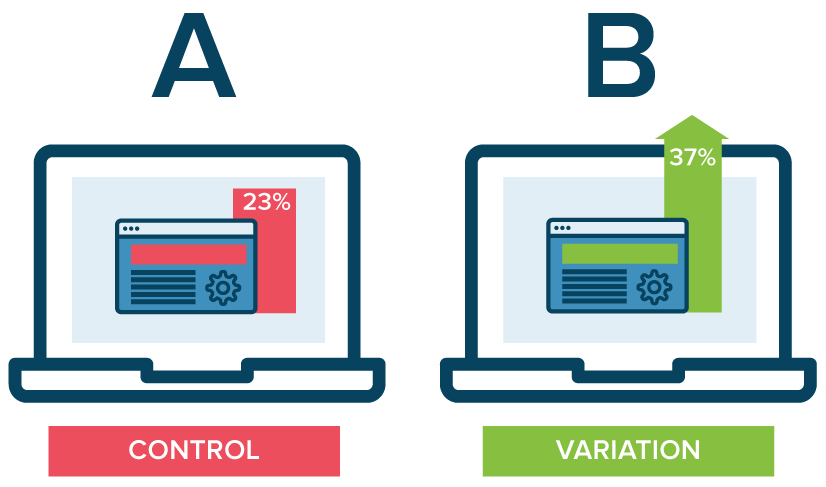
\includegraphics[width=0.9\textwidth]{ab_testing.png}
   			\caption{Принцип A/B тестирования}
    	\end{figure}
    \end{frame}

	\note{A/B тестирование --- это статистический эксперимент, проводящийся путём разделения пользователей на 2 и более группы, представления им различных вариантов продукта и сравнением ключевых показателей. A/B тесты широко применяются как в веб-разработке, так и в разработке мобильных приложений.}
	
	\begin{frame}[fragile]{Дром}
		\begin{figure}[h]
			\centering
			
\includegraphics[width=0.9\textwidth]{drom.png}
			\caption{Дром}
		\end{figure}
	\end{frame}

	\note{
		<<Дром>> --- автомобильный портал, который также является "доской объявлений" о продаже автомобилей. В процессе внесения изменений в портал и мобильные приложения возникает необходимость отслеживать их влияние на метрики продукта. Для этого на <<Дроме>> применяются А/Б тесты.
		\par Тесты проводились вручную, что занимало рабочее время аналитиков, и, тем самым, ограничивало либо количество проводимых тестов, либо их качество.
	}

	\begin{frame}[fragile]{Цель и задачи работы}
		\begin{block}{Цель}
			\ifmetropolis
				\smallskip
			\fi
			Разработка и внедрение системы автоматизированного A/B тестирования в компании <<Дром>>.
		\end{block}
		\begin{block}{Задачи}
			\begin{enumerate}
				\item Провести обзор предметной области;
				\item Провести обзор существующих решений, разработать спецификации нового решения;
				\item Реализовать и внедрить разработанное решение.
			\end{enumerate}
		\end{block}
	\end{frame}
	
	\note{
		Автоматизация A/B тестов позволила бы уменьшить нагрузку на аналитиков, увеличить количество проводимых тестов, ускорить процесс принятия решений и стандартизировать его; дала бы менеджерам возможность непосредственно участвовать в процессе A/B тестирования.
	}
    
    \begin{frame}[fragile]{Анализ существующих решений}
    	\scriptsize
    	\color{black}
		\begin{table}[h]
			\centering
			\begin{tabular}{|p{4cm}|c|c|c|c|c|c|c|c|c|}
			\hline
			& \rot{Google\ } & \rot{Optimizely\ } & \rot{VWO\ } & \rot{Evergage\ } & \rot{Taplytics\ } & \rot{Countly\ } & \rot{Matomo\ } & \rot{Planout\ } & \rot{Sixpack\ }\\
			\hline
			мобильные приложения + веб & 
			\textpm & + & + & + & + & + & + & \textminus & \textminus \\
			\hline
			самостоятельная доработка системы &
			\textminus & \textminus & \textminus & \textminus & \textminus & + & + & + & + \\
			\hline
			анализ сырых данных &
			+ & \textpm & \textpm & + & + & \textpm & \textpm & \textminus & \textminus \\
			\hline
			гибкая настройка метрик &
			\textminus & \textminus & \textminus & \textminus & \textminus & \textminus & \textminus & \textminus & \textminus \\
			\hline 
			хостинг on-premises &
			\textminus & \textminus & \textminus & \textminus & + & + & + & + & + \\
			\hline
			корректный непрерывный мониторинг тестов &
			+ & + & + & + & + & + & \textminus & \textminus & \textminus \\
			\hline
			методики уменьшения дисперсии &
			\textminus & \textminus & \textminus & \textminus & \textminus & \textminus & \textminus & \textminus & \textminus \\
			\hline
			работа с существующими базами данных &
			\textminus & \textminus & \textminus & \textminus & \textminus & \textminus & \textminus & \textminus & \textminus \\
			\hline
			\end{tabular}
			\caption{Сравнительный анализ аналогичных решений}
		\end{table}
    \end{frame}

	\note{Большинство присутствующих на рынке программных продуктов для A/B тестирования являются облачными решениями для аналитики, требующими передачи данных на сервера других компаний; такой формат также не позволяет самостоятельно дорабатывать систему и добавлять новые метрики. Существующие же on-premises решения обладают слабым функционалом, а используемые СУБД не позволяют обрабатывать необходимый объём событий. Решения с исходным кодом позволяют только разделять пользователей на когорты, не содержат функционала анализа результатов.}
	
	\begin{frame}[fragile]{Литература}
		\begin{block}{mSPRT\footnote[1]{
			Peeking at A/B Tests: Why It Matters, and What to Do about It / R. Johari, P.
			Koomen, L. Pekelis, D. Walsh	
		} --- mixture sequential probability ratio test}
			\begin{equation}
				\label{eqn:mSPRT}
				\Lambda_{n}^{H} = \sqrt{\frac{2\sigma^2}{2\sigma^2 +n\tau^2}} \exp\left\{\frac{n^2\tau^2 (\overline{Y}_n-\overline{X}_n)^2}{4\sigma^2(2\sigma^2+n\tau^2)}\right\}
			\end{equation}
			\begin{equation}
				p_0=1;\;p_n=\min\{p_{n-1},1/\Lambda_{n}^{H}\}
			\end{equation}
			%\vspace*{-1cm}
			Где:
			\vspace*{-0.5cm}
			\begin{itemize}
				\item $\sigma$ --- стандартное отклонение объединённой выборки;
				\item $n$ --- объём объединённой выборки;
				\item $\tau$ --- ожидаемый размер эффекта;
				\item $\overline{X}_n,\ \overline{Y}_n$ --- средние двух популяций A/B теста;
				\item $p_i$ --- p-value на шаге $i$.
			\end{itemize}
			\vspace*{-0.5cm}
		\end{block}
		\vfill\null
	\end{frame}
	
	\note{
		В литературе тема A/B тестирования достаточно популярна, хотя основные статистические методы были сформулированы ещё около полувека назад для проведения клинических исследований.
		\par Для корректного непрерывного мониторинга тестов классические статистические критерии, такие как t-тест Стьюдента не подходят, и необходимо использовать специально предназначенные для этого методы, такие как mSPRT. Этот тест требует знания точной формы распределения --- например нормальное, или Бернулли.
	}

	\begin{frame}[fragile]{Литература}
		\begin{block}{Bootstrap mSPRT\footnote[2]{
					Abhishek V., Mannor S. A Nonparametric Sequential Test for Online Randomized
Experiments
			}}
			\ifmetropolis
				\smallskip
			\fi
			\begin{itemize}
				\item распределение данных заранее неизвестно;
				\item функция правдоподобия заменяется эмпирической оценкой по данным;
				\item используется бутстрап.
			\end{itemize}
		\end{block}
		\vfill\null
	\end{frame}

	\note{
		Модификация данного метода позволяет применять его для любого заранее неизвестного распределения, эмпирически оценивая функцию правдоподобия, используя бутстрап. Это необходимо для многих метрик, особенно связанных с финансами.
	}

	\begin{frame}[fragile]{Литература}
		\begin{block}{Уменьшение дисперсии с использованием CatBoost\footnote[3]{
					Boosted Decision Tree Regression Adjustment for Variance Reduction in Online
Controlled Experiments / A. Poyarkov, A. Drutsa, A. Khalyavin, G. Gusev, P.
Serdyukov
			}}
			\ifmetropolis
			\smallskip
			\fi
			\begin{equation}
				\tilde{Y}=F(X)
			\end{equation}
			\begin{equation}
				\overset{\triangle}{Y}=Y-\tilde{Y}
			\end{equation}
			\begin{equation}
				\text{ATE}(\overset{\triangle}{Y})=\text{ATE}(Y)
			\end{equation}
			\begin{equation}
				\text{var}(\overset{\triangle}{Y})=\text{var}(Y)-\text{var}(\tilde{Y})
			\end{equation}
		\end{block}
		\vfill\null
	\end{frame}
	
	\note{
		Уменьшение дисперсии позволяет значительно сократить время проведения A/B теста. Работа сотрудников Яндекс предлагает предсказывать значение метрики, используя CatBoost, тем самым <<объясняя>> часть дисперсии и уменьшая влияние сторонних факторов на эксперимент. При этом разница между когортами остаётся неизменной.
	}

	\begin{frame}[fragile]{Структура проекта}
		\begin{figure}[h]
			\centering
			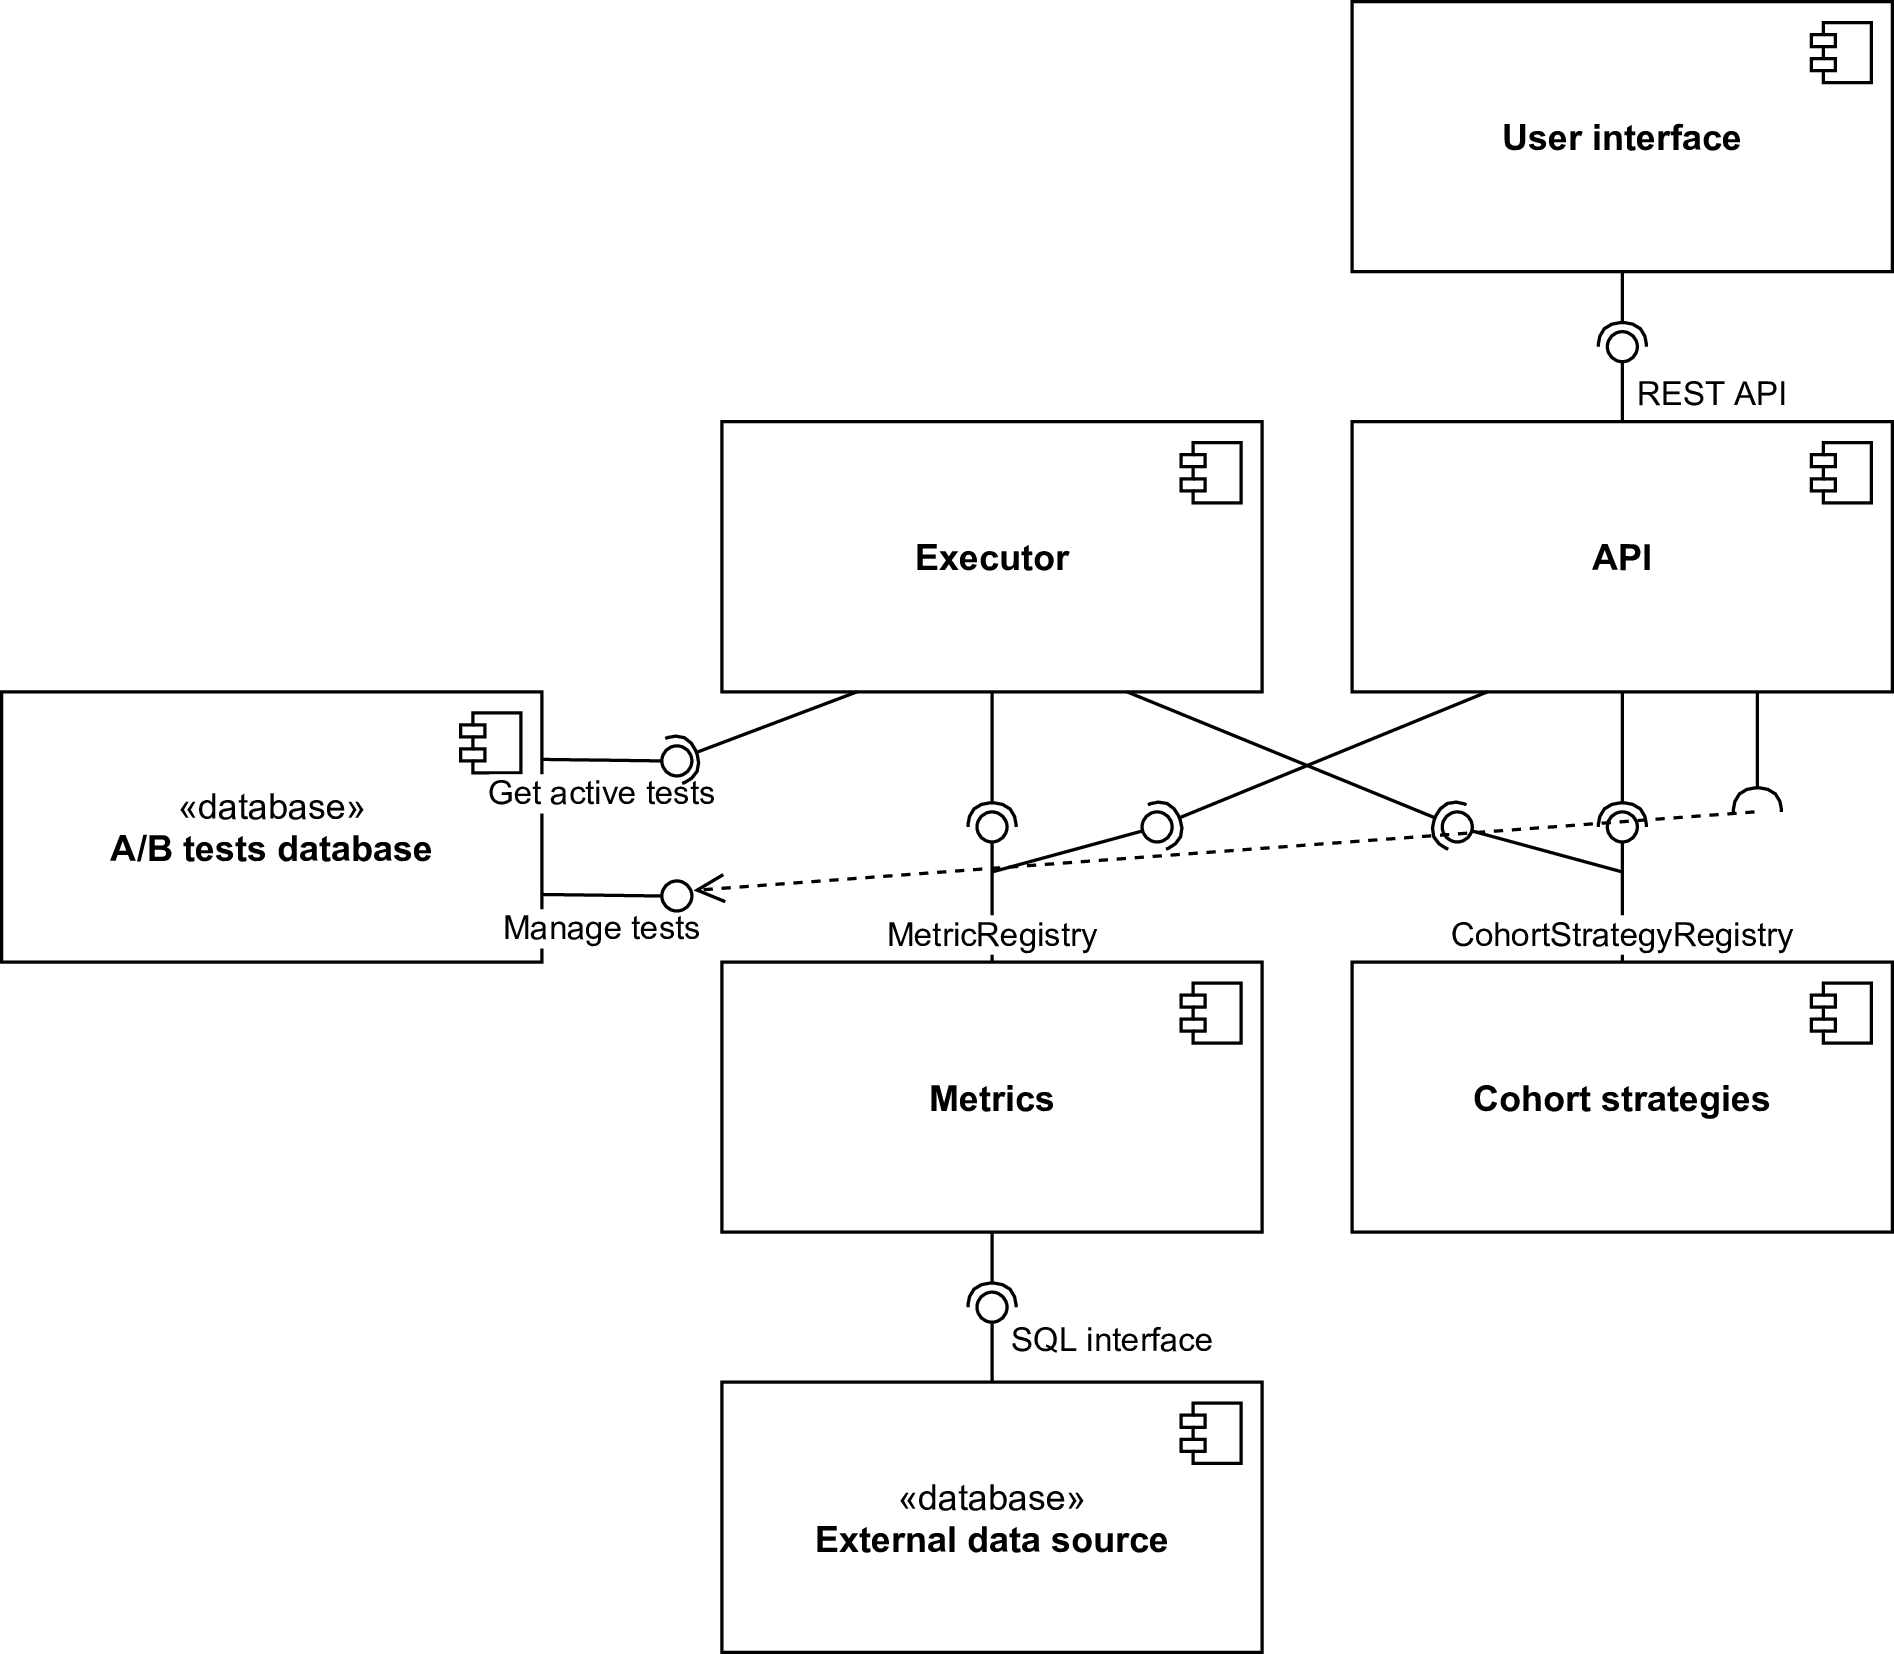
\includegraphics[width=0.6\textwidth]{component_diagram.png}
			\caption{Диаграмма компонентов}
		\end{figure}
	\end{frame}

	\note{
		На <<Дроме>> уже существовала система управления A/B тестами (но не анализа результатов), поэтому разработка была сконцентрирована именно в области корректного мониторинга и анализа результатов тестов.
		\par Архитектурно система состоит из Executor-a, исполняющего тесты по расписанию, и пользовательского интерфейса, через который осуществляется управление тестами и просмотр их результатов. Остальные части системы представляют собой их общие зависимости: метрики, стратегии разделения на когорты, база данных с результатами тестов, реализованные математические методы.
	}

	\begin{frame}[fragile]{Принятые решения}
		\begin{block}{}
			\begin{itemize}
				\item метрики содержат любые вычисления, модульны;
				\item стратегии распределения по когортами модульны;
				\item генерация формы создания теста по схеме;
				\item Executor и API --- отдельные сервисы;
				\item Kubernetes для развёртывания;
				\item bootstrap mSPRT на C++;
			\end{itemize}
		\end{block}
	\end{frame}

	\note{
		В связи с разнообразием как метрик, применяемых на <<Дроме>>, так и методов разделения пользователей на когорты, было принято решение реализовать их как независимые автоматически регистрируемые модули.
		\par Для добавления новых тестов через графический интерфейс в условиях постоянного добавления новых модулей была реализована автоматическая генерация формы создания A/B теста.
		\par Executor и API были развёрнуты в виде двух сервисов в Kubernetes для удобства логирования и обеспечения в будущем возможности развернуть несколько Executor-ов.
		\par Из-за высокой вычислительной сложности критерий bootstrap mSPRT был реализован на C++ в виде расширения для Python;
	}
    
	\begin{frame}[fragile]{Интерфейс}
		\begin{figure}[h]
			\centering
			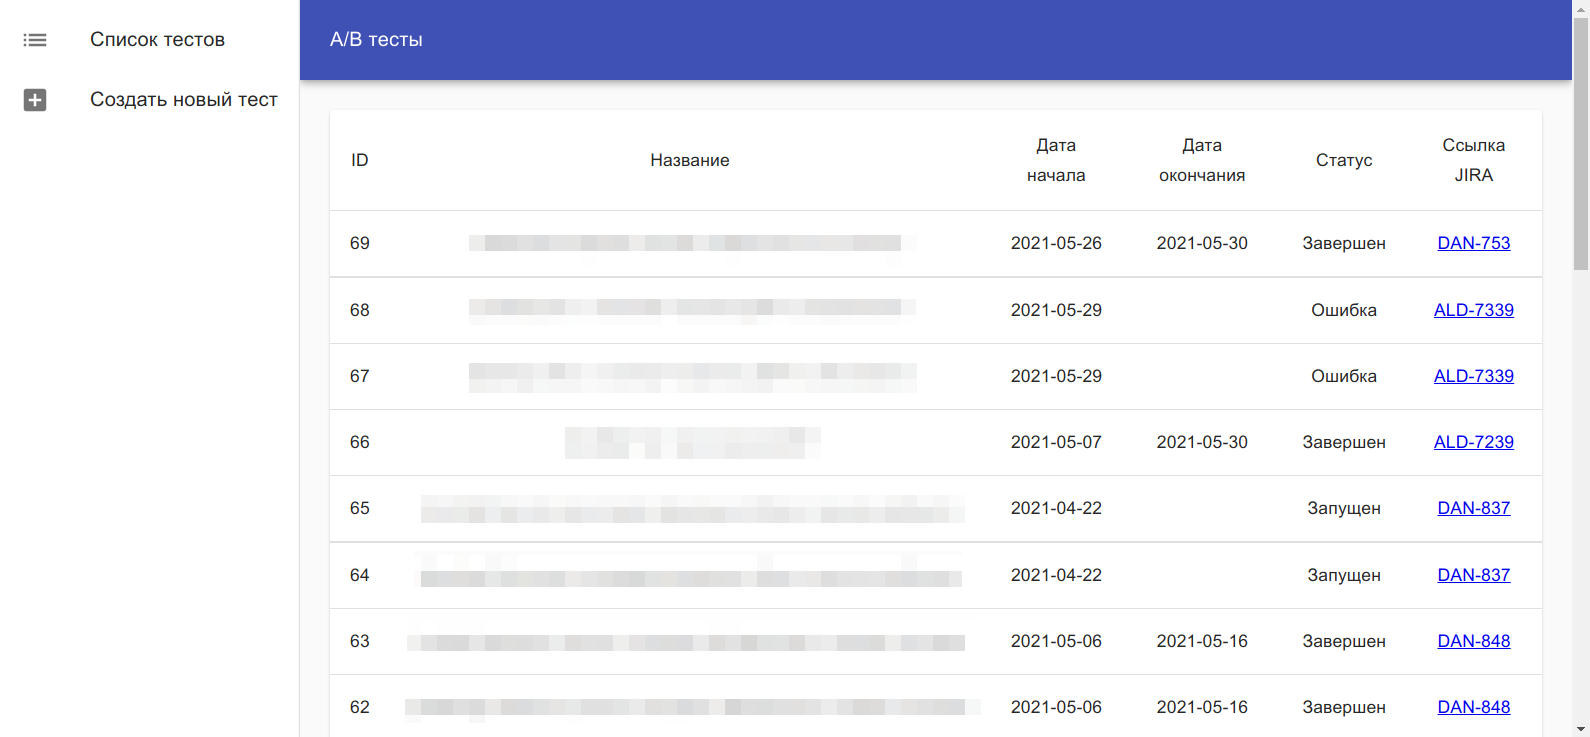
\includegraphics[width=\textwidth]{main_page.png}
			\caption{Страница списка A/B тестов}
		\end{figure}
	\end{frame}

	\note{
		На текущий момент менеджерами с использованием системы было проведено 68 A/B тестов, в результате чего было сэкономлено около 550 часов работы аналитиков.
	}

	\begin{frame}[fragile]{Итоги}
		\begin{block}{}
			\begin{itemize}
				\item Успешно разработана и внедрена система автоматизированного A/B тестирования в компании <<Дром>>;
				\item Система использует корректные методы тестирования статистических гипотез и методики понижения дисперсии;
				\item В результате внедрения системы была снижена нагрузка на аналитиков данных и выросло количество проводимых A/B тестов;
			\end{itemize}
		\end{block}
	\end{frame}

	\note{
		Читаем со слайда. Спасибо за внимание.
	}
    
\end{document}